\part{CSS}

\newpage

\chapter{CSS简介}

\section{给HTML打扮——CSS样式}

\subsection{层叠样式表(CSS, Cascading Style Sheets)}

CSS用于定义HTML内容在浏览器内的显示样式,如文字大小、颜色、字体加粗等。使用CSS的好处是通过定义某个样式,可以让网页不同位置的文本有统一的字体、字号或颜色等。CSS由选择器和声明组成,而声明又由属性和值组成。 \\

选择器用于指明网页中要应用样式规则的元素。声明的内容写在大括号内,属性和值之前用【:】分隔。当有多条声明时,中间可以用【;】分隔。为了使样式更加容易阅读,可以将每条声明单独成行。 \\

\mybox{修改字体大小和颜色} \\
\begin{lstlisting}[style=htmlcssjs]
<!DOCTYPE html>
<html lang="en">
<head>
    <meta charset="UTF-8">
    <title>修改字体大小和颜色</title>
    <style type="text/css">
        p {
            font-size: 20px;
            color: red;
        }
    </style>
</head>
<body>
    <p>修改字体大小和颜色</p>
</body>
</html>
\end{lstlisting}

\newpage

\section{既然那么好,那就引入CSS吧——内联式CSS}

\subsection{内联式CSS}

内联式CSS样式,也称行间样式,就是把CSS代码直接写在现有的HTML标签中。注意CSS样式必须写在元素的开始标签里,不能在结束标签里。 \\

\begin{lstlisting}[style=htmlcssjs]
<开始标签 style="属性: 值;">文本</结束标签>
\end{lstlisting}

CSS样式必须写在style属性的双引号中,如果有多条CSS样式代码可以设置可以写在一起,中间用【;】隔开。 \\

\mybox{内联式CSS} \\
\begin{lstlisting}[style=htmlcssjs]
<!DOCTYPE html>
<html lang="en">
<head>
    <meta charset="UTF-8">
    <title>内联式CSS</title>
</head>
<body>
    <p style="color: red; font-size: 20px;">内联式CSS</p>
</body>
</html>
\end{lstlisting}

\newpage

\section{换个地方吧,行内太挤了——嵌入式CSS}

\subsection{嵌入式CSS}

嵌入式CSS样式,也称页面级CSS样式,就是把CSS样式代码写在<style>之间,嵌入式CSS样式一般放在<head>内。 \\

\mybox{嵌入式CSS} \\
\begin{lstlisting}[style=htmlcssjs]
<!DOCTYPE html>
<html lang="en">
<head>
    <meta charset="UTF-8">
    <title>嵌入式CSS</title>
    <style type="text/css">
        span {
            color: red;
        }
    </style>
</head>
<body>
    <p><span>乔恩</span>找到<span>艾洛莉</span></p>
</body>
</html>
\end{lstlisting}

\newpage

\section{还是把HTML和CSS分开吧——外部式CSS}

\subsection{外部式CSS}

外部式CSS样式,也称外联式CSS样式,就是把CSS样式代码写一个单独的外部文件中,这个CSS样式文件以.css为扩展名。在<head>内使用<link>将CSS外部样式文件链接到HTML文件内。 \\

\begin{lstlisting}[style=htmlcssjs]
<link href="CSS样式文件名" rel="stylesheet" type="text/css" />
\end{lstlisting}

CSS样式文件名以有意义的英文命名,<link>中\lstinline|rel="stylesheet" type="text/css"|是固定写法,不需要修改。 \\

\mybox{外部式CSS}
\begin{lstlisting}[style=htmlcssjs, title=external\_css.html]
<!DOCTYPE html>
<html lang="en">
<head>
    <meta charset="UTF-8">
    <title>外部式CSS</title>
    <link type="text/css" rel="stylesheet" href="external_css.css">
</head>
<body>
    <div></div>
</body>
</html>
\end{lstlisting}

\begin{lstlisting}[style=htmlcssjs, title=external\_css.css]
div {
    width: 100px;
    height: 100px;
    background-color: blue;
}
\end{lstlisting}

\newpage

\section{总有个先来后到吧——三种链接方式的优先级}

\subsection{CSS引入方式优先级}

如果有一种情况:对于同一个元素同时使用了三种方法设置CSS样式,那么哪种方式真正有效呢? \\

三种CSS引入方式是有优先级的:内联式 > 嵌入式 > 外部式。但是嵌入式 > 外部式有一个前提,那就是嵌入式CSS样式的位置一定在外部式的后面。在实际开发中也会将<link>写在<style>的前面。 \\

总的来说,优先级遵循“就近原则”,离被设置元素越近优先级别越高。 \\

但是以上总结的优先级有一个前提,那就是内联式、嵌入式、外部式样式表中CSS样式是在相同权值的情况下。那权值是什么呢?

\begin{figure}[H]
	\centering
	
\includegraphics[]{img/C5/5-5/1.png}
\end{figure}

\newpage

\chapter{选择器}

\section{选一个标签——标签选择器}

\subsection{标签选择器}

标签选择器其实就是HTML代码中的标签。 \\

\begin{lstlisting}[style=htmlcssjs]
tag_selector {
    attribute: value;
}
\end{lstlisting}

\vspace{0.5cm}
\mybox{标签选择器} \\
\begin{lstlisting}[style=htmlcssjs]
<!DOCTYPE html>
<html lang="en">
<head>
    <meta charset="UTF-8">
    <title>标签选择器</title>
    <style type="text/css">
        h2 {
            color: green;
            font-size: 30px;
        }
    </style>
</head>
<body>
    <h2>CSS特点</h2>
    <p>CSS为HTML标记语言提供了一种样式描述。</p>
</body>
</html>
\end{lstlisting}

\newpage

\section{再选一个类——类选择器}

\subsection{类选择器}

类选择器在CSS样式中是最常用的。类选择器使用【.】开头,后加类选择器的名称,CSS样式代码会被作用到属于该类的HTML标签中。在标签中使用class属性为标签设置一个类。 \\

类选择器与标签是多对多的关系,即类选择器名称可以多个标签共用,一个元素可以用多个class,一个class值可以对应多个元素。多个class值之间使用空格分隔。 \\

\mybox{类选择器} \\
\begin{lstlisting}[style=htmlcssjs]
<!DOCTYPE html>
<html lang="en">
<head>
    <meta charset="UTF-8">
    <title>类选择器</title>
    <style type="text/css">
        .title {
            color: green;
        }
    </style>
</head>
<body>
    <h3 class="title">丰富的样式定义</h3>
    <p>CSS提供了丰富的文档样式外观。</p>
    <h3 class="title">易于使用和修改</h3>
    <p>CSS样式表可以将所有的样式声明统一存放,进行统一管理。</p>
</body>
</html>
\end{lstlisting}

\newpage

\section{取个唯一表示——ID选择器}

\subsection{ID选择器}

使用ID选择器,必须给标签添加上id属性,即为标签设置id属性。ID选择器名称的前面使用【\#】。ID选择器与标签是一对一的关系,即一个元素只能有一个id值,一个id值只能对应一个元素。id是全局唯一的,就像身份证号码一样。 \\

\mybox{ID选择器} \\
\begin{lstlisting}[style=htmlcssjs]
<!DOCTYPE html>
<html lang="en">
<head>
    <meta charset="UTF-8">
    <title>ID选择器</title>
    <style type="text/css">
        div {
            width: 100px;
            height: 100px;
        }

        #square1 {
            background-color: red;
        }
        #square2 {
            background-color: blue;
        }
    </style>
</head>
<body>
    <div id="square1"></div>
    <div id="square2"></div>
</body>
</html>
\end{lstlisting}

\newpage

\section{捡了个儿子——子选择器}

\subsection{子选择器}

子选择器【>】,用于选择指定标签元素的第一代子元素。 \\

\mybox{子选择器} \\
\begin{lstlisting}[style=htmlcssjs]
<!DOCTYPE html>
<html lang="en">
<head>
    <meta charset="UTF-8">
    <title>子选择器</title>
    <style type="text/css">
        .food > li {
            border: 1px solid red;
        }
    </style>
</head>
<body>
    <h2>食物</h2>
    <ul class="food">
        <li>水果
            <ul>
                <li>苹果</li>
            </ul>
        </li>
        <li>蔬菜
            <ul>
                <li>白菜</li>
            </ul>
        </li>
    </ul>
</body>
</html>
\end{lstlisting}

\newpage

\section{这么快就当爷爷了——后代选择器}

\subsection{后代选择器}

后代选择器,也称包含选择器,用于选择指定标签元素的后辈元素。 \\

\begin{lstlisting}[style=htmlcssjs]
ancestor_selector descendant_selector {
    attribute: value;
}
\end{lstlisting}

后代选择器与子选择器的区别在于,子选择器仅是指它的直接后代,而后代选择器是作用于所有子后代元素。 \\

\mybox{后代选择器} \\
\begin{lstlisting}[style=htmlcssjs]
<!DOCTYPE html>
<html lang="en">
<head>
    <meta charset="UTF-8">
    <title>后代选择器</title>
    <style type="text/css">
        .food li {
            border: 1px solid red;
        }
    </style>
</head>
<body>
    <h2>食物</h2>
    <ul class="food">
        <li>
            水果
            <ul>
                <li>苹果</li>
                <li>香蕉</li>
                <li>橘子</li>
            </ul>
        </li>
        <li>
            蔬菜
            <ul>
                <li>白菜</li>
                <li>油菜</li>
                <li>卷心菜</li>
            </ul>
        </li>
    </ul>
</body>
</html>
\end{lstlisting}

\newpage

\section{我全都要——通配符选择器}

\subsection{通配符选择器}

通配符选择器【*】,也称通用选择器,是功能最强大的选择器,用于匹配HTML中所有的标签元素,包括<html>、<body>等。 \\

\mybox{通配符选择器} \\
\begin{lstlisting}[style=htmlcssjs]
<!DOCTYPE html>
<html lang="en">
<head>
    <meta charset="UTF-8">
    <title>通配符选择器</title>
    <style type="text/css">
        * {
            background-color: yellow;
        }
    </style>
</head>
<body>

</body>
</html>
\end{lstlisting}

\newpage

\section{给选择器分个组——分组选择器}

\subsection{分组选择器}

分组选择器【,】,用于为HTML中多个标签元素设置同一个样式。 \\

\mybox{分组选择器} \\
\begin{lstlisting}[style=htmlcssjs]
<!DOCTYPE html>
<html lang="en">
<head>
    <meta charset="UTF-8">
    <title>分组选择器</title>
    <style type="text/css">
        h1, h2, h3 {
            color: red;
        }
    </style>
</head>
<body>
    <h1>HTML</h1>
    <h2>CSS</h2>
    <h3>JavaScript</h3>
</body>
</html>
\end{lstlisting}

\newpage

\section{伪装者——伪类选择器}

\subsection{伪类选择器}

伪类选择器【:】允许给HTML标签的某种状态设置样式,例如给一个标签元素的鼠标滑过的状态设置字体颜色。

\begin{table}[H]
	\centering
	\setlength{\tabcolsep}{5mm}{
		\begin{tabular}{|c|c|}
			\hline
			\textbf{伪类选择器} & \textbf{功能}    \\
			\hline
			:link               & 未访问           \\
			\hline
			:visited            & 已访问           \\
			\hline
			:hover              & 鼠标悬停         \\
			\hline
			:active             & 鼠标按下         \\
			\hline
			:enabled            & 可用的时候触发   \\
			\hline
			:disabled           & 不可用的时候触发 \\
			\hline
		\end{tabular}
	}
	\caption{常用伪类选择器}
\end{table}

到目前为止,可以兼容所有浏览器的伪类选择器就是在<a>上使用:hover。 \\

\mybox{伪类选择器} \\
\begin{lstlisting}[style=htmlcssjs]
<!DOCTYPE html>
<html lang="en">
<head>
    <meta charset="UTF-8">
    <title>伪类选择器</title>
    <style type="text/css">
        a:hover {
            color: orange;
        }
    </style>
</head>
<body>
    <a href="http://www.baidu.com">百度一下,你就知道</a>
</body>
</html>
\end{lstlisting}

\newpage

\section{为所欲为——选择器最高层级!important}

\subsection{选择器优先级}

每个选择器都是有优先级的,如果一个元素使用了多个选择器,则会按照选择器的优先级来给定样式。 \\

选择器的优先级依次是:内联样式 > ID选择器 > 类选择器 > 标签选择器 > 通配符选择器。

\subsection{选择器权重}

浏览器是根据权值来判断使用哪种CSS样式的,权值高的优先级更高。

\begin{table}[H]
	\centering
	\setlength{\tabcolsep}{5mm}{
		\begin{tabular}{|c|c|}
			\hline
			\textbf{选择器} & \textbf{权值} \\
			\hline
			!important      & $ \infty $    \\
			\hline
			行间样式        & 1000          \\
			\hline
			ID              & 100           \\
			\hline
			class           & 10            \\
			\hline
			标签            & 1             \\
			\hline
			通配符          & 0             \\
			\hline
		\end{tabular}
	}
	\caption{选择器权重}
\end{table}

\subsection{!important}

有些特殊情况需要为某些样式设置具有最高权值,这时候可以使用!important,注意!important要写在分号的前面。 \\

\mybox{!important} \\
\begin{lstlisting}[style=htmlcssjs]
<!DOCTYPE html>
<html lang="en">
<head>
    <meta charset="UTF-8">
    <title>!important</title>
    <style type="text/css">
        h1 {
            color: red !important;
        }

        h1 {
            color: blue;
        }
    </style>
</head>
<body>
    <h1>为所欲为</h1>
</body>
</html>
\end{lstlisting}

\newpage

\chapter{字体、文本样式}

\section{字体样式}

\subsection{字体样式}

使用CSS样式可以为网页中的文字设置字体。注意不要设置不常用的字体,因为如果用户本地电脑上没有安装该字体,就会显示浏览器默认的字体。 \\

浏览器默认的字号为16px,使用font-size可以修改字号大小。 \\

为文字设置粗体是有单独的CSS样式来实现的,再也不用为了实现粗体样式而使用<h1>-<h6>或<strong>了。 \\

font-weight的默认值为normal,通过设置属性值为lighter、bold、bolder或100-900之间的整百数值改变文字的粗细。注意,字体能否被bolder或lighter更改取决于字体包是否存在该样式。 \\

font-style可以设置字体样式,并且有3种设置方式:

\begin{enumerate}
	\item 正常字体为normal,也是font-style的默认值
	\item italic为字体设置为斜体,用于字体本身就有倾斜的样式
	\item oblique强制将字体倾斜
\end{enumerate}

\mybox{字体样式} \\
\begin{lstlisting}[style=htmlcssjs]
<!DOCTYPE html>
<html lang="en">
<head>
    <meta charset="UTF-8">
    <title>字体样式</title>
    <style type="text/css">
        p {
            font-family: "arial";
            font-size: 20px;
            font-weight: bold;
            font-style: italic;
        }   
    </style>
</head>
<body>
    <p>Cascading Style Sheets (CSS) is a style sheet language used for describing the presentation of a document written in a markup language such as HTML.</p>
</body>
</html>
\end{lstlisting}

\newpage

\section{上个色——color}

\subsection{color}

color属性可以设置字体颜色。color的值有3种设置方式:

\begin{enumerate}
	\item 英文命令颜色。 \\
	      \begin{lstlisting}[style=htmlcssjs]
color: red;
    \end{lstlisting}

	\item 十六进制颜色代码:使用6位十六进制数表示光学三原色“红绿蓝”。
	      \begin{table}[H]
		      \centering
		      \setlength{\tabcolsep}{5mm}{
			      \begin{tabular}{|c|c|c|}
				      \hline
				      \textbf{R} & \textbf{H} & \textbf{B} \\
				      \hline
				      00 - FF    & 00 - FF    & 00 - FF    \\
				      \hline
			      \end{tabular}
		      }
		      \caption{颜色代码}
	      \end{table}
	      如果每两位十六进制数都相同,可简写。
	      \begin{table}[H]
		      \centering
		      \setlength{\tabcolsep}{5mm}{
			      \begin{tabular}{|c|c|}
				      \hline
				      \textbf{颜色代码} & \textbf{颜色} \\
				      \hline
				      \#F00             & 红色          \\
				      \hline
				      \#0F0             & 绿色          \\
				      \hline
				      \#00F             & 蓝色          \\
				      \hline
				      \#000             & 黑色          \\
				      \hline
				      \#FFF             & 白色          \\
				      \hline
				      \#0FF             & 青色          \\
				      \hline
				      \#F40             & 淘宝红        \\
				      \hline
			      \end{tabular}
		      }
		      \caption{常见颜色代码}
	      \end{table}

	\item 颜色函数rgb():由光学三原色RGB的比例来配色。rgb()函数中每一项的值可以是0-255之间的整数,也可以是0\%-100\%的百分数。 \\
	      \begin{lstlisting}[style=htmlcssjs]
color: rgb(133, 45, 200);
color: rgb(20%, 33%, 25%);
    \end{lstlisting}
\end{enumerate}

\newpage

\section{文本样式}

\subsection{文本样式}

使用text-decoration可以设置对文本的修饰,默认值为none;属性值为underline为下划线,属性值为overline为上划线,属性值为line-through为穿过文本的线,一般用于商品折扣价。使用line-height可以设置段落中的行间距离(行高)。使用text-align可以为文本设置对齐方式,属性值包括left、right和center。 \\

\mybox{文本样式} \\
\begin{lstlisting}[style=htmlcssjs]
<!DOCTYPE html>
<html lang="en">
<head>
    <meta charset="UTF-8">
    <title>文本样式</title>
    <style type="text/css">
        h2, p {
            text-decoration: underline;
            line-height: 2em;   /* 两倍行间距 */
            text-align: center;
        }
    </style>
</head>
<body>
    <h2>《望庐山瀑布》</h2>
    <p>唐·李白</p>
    <p>
        日照香炉生紫烟,<br/>
        遥看瀑布挂前川。<br/>
        飞流直下三千尺,<br/>
        疑是银河落九天。
    </p>
</body>
</html>
\end{lstlisting}

\newpage

\chapter{盒子模型与布局模型}

\section{元素分类}

\subsection{我要独占一行——块级元素}

在HTML中<div>、<p>、<h1>、<form>、<ul>、<li>等都是块级元素。每个块级元素都从新的一行开始,并且其后的元素也另起一行。块级元素的高度、宽度、行高遗迹顶和底边距都可以设置,宽度在不设定的情况下,是它本身父容器的100\%(和父元素的宽度一致)。 \\

\mybox{块级元素} \\
\begin{lstlisting}[style=htmlcssjs]
<!DOCTYPE html>
<html lang="en">
<head>
    <meta charset="UTF-8">
    <title>块级元素</title>
</head>
<body>
    <div>这是一个div标签</div>
    <p>这是一个p标签</p>
    <h1>这是一个h1标签</h1>
</body>
</html>
\end{lstlisting}

通过设置\lstinline|display: block|可以将元素显示为块级元素。

\subsection{我要和你站一起——内联元素}

在HTML中,<span>、<a>、<label>、<strong>、<em>等都是内联元素(行内元素)。内联元素和其它元素都在一行上,元素的高度、宽度及顶部和底部编剧不可设置,元素的宽度就是它包含的文字或图片的宽度,不可改变。 \\

块级元素也可以设置\lstinline|display: inline|将元素设置为内联元素。 \\

\mybox{内联元素与块级元素转换} \\
\begin{lstlisting}[style=htmlcssjs]
<!DOCTYPE html>
<html lang="en">
<head>
    <meta charset="UTF-8">
    <title>内联元素与块级元素转换</title>
    <style type="text/css">
        a {
            display: block;
        }

        div {
            display: inline;
        }
    </style>
</head>
<body>
    <a>我要变成块级元素</a>
    <a>我也要变成块级元素</a>
    <div>我要变成内联元素</div>
    <div>我也要变成内联元素</div>
</body>
</html>
\end{lstlisting}

\subsection{我还要占个大位置——内联块状元素}

内联块状元素就是同时具备内联元素和块级元素的特点。内联块状元素的特点是和其它元素都在一行上,但元素的高度、宽度、行高以及顶和底边距都可以设置。 \\

通过设置\lstinline|display: inline-block|就可以将元素设置为内联块状元素。如<img>、<input>就是这种内联块状标签。

\newpage

\section{盒子模型}

\subsection{盒子模型}

盒子模型包含4个部分:

\begin{enumerate}
	\item 外边距(margin)
	\item 外边框(border)
	\item 内边距(padding)
	\item 内容(content)
\end{enumerate}

\begin{figure}[H]
	\centering
	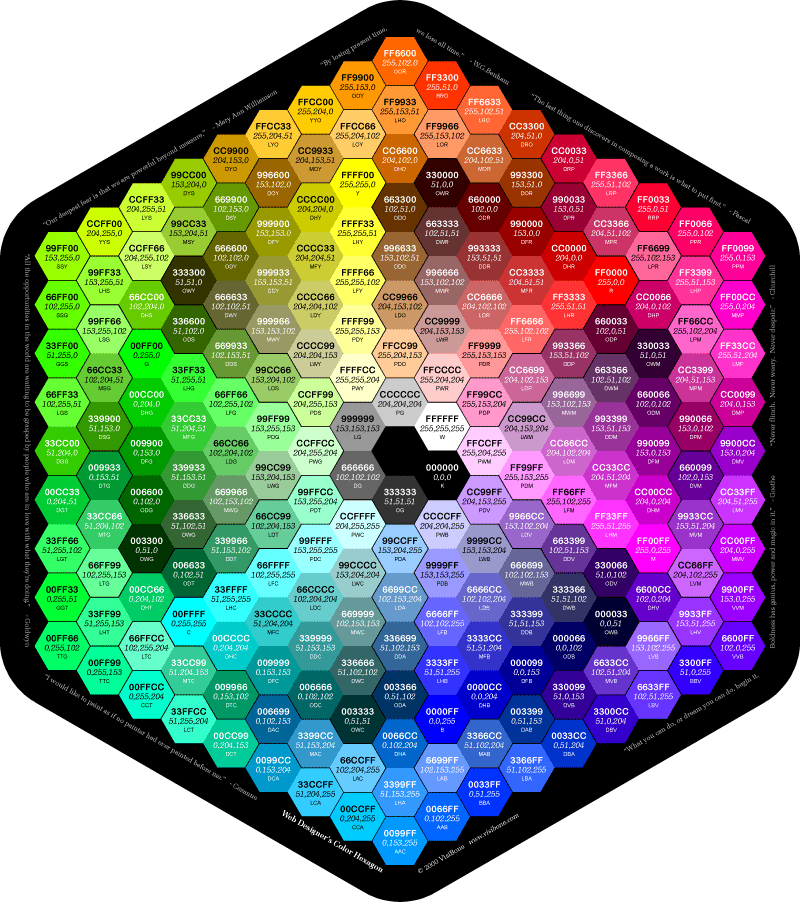
\includegraphics[scale=0.7]{img/C8/8-2/1.png}
\end{figure}

盒模型的宽度和高度和平常所说的物体的宽度和高度的理解是不一样的,CSS内定义的宽和高,指的是盒模型中内容的宽和高。 \\

元素实际的宽度(盒子的宽度) = 左外边距 + 左边框 + 左内边距 + 内容宽度 + 右内边距 + 右边框 + 右外边距 \\

\begin{figure}[H]
	\centering
	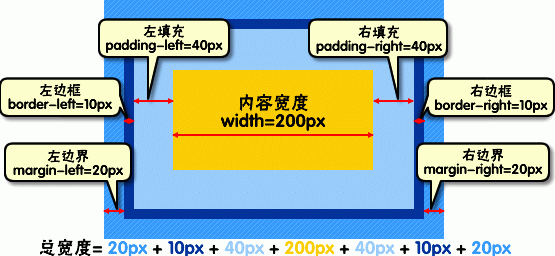
\includegraphics[]{img/C8/8-2/2.png}
\end{figure}

\subsection{外边框(Border)}

盒子模型的外边框可以设置粗细、样式和颜色:

\begin{enumerate}
	\item border-width:设置边框的宽度,常用单位为像素(px)
	\item border-style:边框样式包括实线solid、虚线dashed、点线dotted
	\item border-color:设置边框颜色
\end{enumerate}

当三个属性都需要被设置时,也可以使用border属性简写。例如设置一个粗细为1px实心的黑色边框: \\

\begin{lstlisting}[style=htmlcssjs]
border: 1px solid black;
\end{lstlisting}

CSS中也允许只为一个方向的边框设置属性,使用border-top、border-bottom、border-left、border-right可以单独设置上、下、左、右四条边框。 \\

元素边框的圆角效果可以使用border-radius属性来设置。设置圆角的值的顺序为左上、右上、右下、左下。如果border-radius属性只给出一个值表示四个圆角都被设置成该值。如果只给出两个值表示左上角和右下角设置为第一个值,右上角和左下角设置为第二个值。当给一个正方形的圆角效果值设置为其宽度一半时,显示效果为圆形。 \\

\mybox{圆形} \\
\begin{lstlisting}[style=htmlcssjs]
<!DOCTYPE html>
<html lang="en">
<head>
    <meta charset="UTF-8">
    <title>圆形</title>
    <style type="text/css">
        div {
            width: 100px;
            height: 100px;
            background-color: red;
            border-radius: 50%;
        }
    </style>
</head>
<body>
    <div></div>
</body>
</html>
\end{lstlisting}

通过单独设置每条边的属性,可以在正方形内展现不同的颜色。

\begin{figure}[H]
	\centering
	\begin{tikzpicture}
		\filldraw[draw=black, fill=black] (0,0) -- (5,0) -- (2.5,2.5) -- cycle;
		\filldraw[draw=red, fill=red] (0,0) -- (2.5,2.5) -- (0,5) -- cycle;
		\filldraw[draw=blue, fill=blue] (5,0) -- (2.5,2.5) -- (5,5) -- cycle;
		\filldraw[draw=green, fill=green] (2.5,2.5) -- (0,5) -- (5,5) -- cycle;
	\end{tikzpicture}
\end{figure}

\mybox{四色正方形} \\
\begin{lstlisting}[style=htmlcssjs]
<!DOCTYPE html>
<html lang="en">
<head>
    <meta charset="UTF-8">
    <title>四色正方形</title>
    <style type="text/css">
        div {
            width: 0;
            height: 0;
            border: 100px solid black;
            border-left-color: red;
            border-top-color: green;
            border-right-color: blue;
        }
    </style>
</head>
<body>
    <div></div>
</body>
</html>
\end{lstlisting}

通过设置透明色(transparent),可以绘制出三角形。

\begin{figure}[H]
	\centering
	\begin{tikzpicture}
		\filldraw[draw=black, fill=black] (0,0) -- (5,0) -- (2.5,2.5) -- cycle;
		\filldraw[draw=black, fill=black] (0,0) -- (2.5,2.5) -- (0,5) -- cycle;
	\end{tikzpicture}
\end{figure}

\mybox{三角形} \\
\begin{lstlisting}[style=htmlcssjs]
<!DOCTYPE html>
<html lang="en">
<head>
    <meta charset="UTF-8">
    <title>三角形</title>
    <style type="text/css">
        div {
            width: 0;
            height: 0;
            border: 100px solid black;
            border-left-color: black;
            border-top-color: transparent;
            border-right-color: transparent;
        }
    </style>
</head>
<body>
    <div></div>
</body>
</html>
\end{lstlisting}

\subsection{内边距(Padding)}

元素内容与边框之间是可以设置距离的,称之为内边距或填充。内边距也可分为上、右、下、左(顺时针)。

\begin{figure}[H]
	\centering
	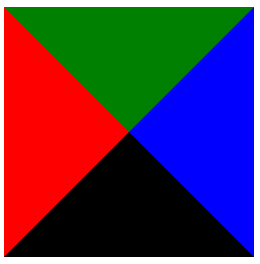
\includegraphics[scale=0.7]{img/C8/8-2/3.png}
\end{figure}

\subsection{外边距(Margin)}

元素与其他元素之间的距离可以使用外边距来设置,外边距也可分为上、右、下、左。

\begin{figure}[H]
	\centering
	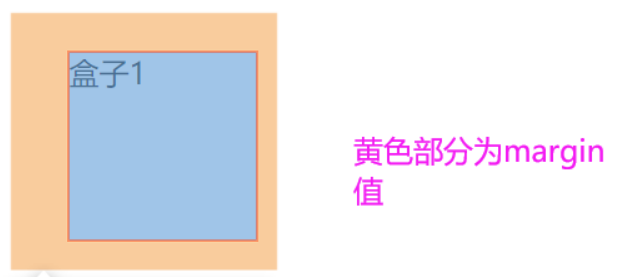
\includegraphics[scale=0.7]{img/C8/8-2/4.png}
\end{figure}

margin与padding的区别在于,padding在外边框里,margin在外边框外。

\newpage

\section{布局模型}

\subsection{布局模型}

布局模型建立在盒子模型的基础上,在网页中,元素有3种布局模型:

\begin{enumerate}
	\item 流动模型(flow)
	\item 浮动模型(float)
	\item 层模型(layer)
\end{enumerate}

\subsection{流动模型}

流动模型是默认的网页布局模式,也就是说网页在默认状态下的HTML网页元素都是根据流动模型来分布网页内容的。 \\

流动布局模型有2个典型的特征:

\begin{enumerate}
	\item 块级元素都会在所处的包含元素内自上而下按顺序垂直延伸分布,因为在默认状态下,块级元素的宽度都为100\%,即都会以行的形式占据位置。
	      \begin{figure}[H]
		      \centering
		      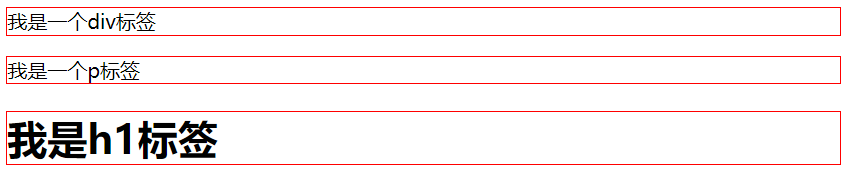
\includegraphics[scale=0.7]{img/C8/8-3/1.png}
	      \end{figure}

	\item 内联元素都会在所处的包含元素内从左到右水平分布显示。
	      \begin{figure}[H]
		      \centering
		      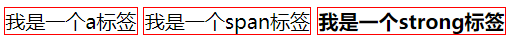
\includegraphics[]{img/C8/8-3/2.png}
	      \end{figure}
\end{enumerate}

\subsection{浮动模型}

块级元素这么霸道都是独占一行,如果想让两个块级元素并排显示,可以设置元素浮动。任何元素在默认情况下是不能浮动的,但可以设置float属性定义为浮动,如<div>、<p>、<table>、<img>等元素都可以被定义为浮动。 \\

\mybox{浮动模型} \\
\begin{lstlisting}[style=htmlcssjs]
<!DOCTYPE html>
<html lang="en">
<head>
    <meta charset="UTF-8">
    <title>浮动模型</title>
    <style type="text/css">
        div {
            width: 100px;
            height: 100px;
            border: 1px solid red;
        }

        #div1 {
            float: left;
        }

        #div2 {
            float: right;
        }
    </style>
</head>
<body>
    <div id="div1"></div>
    <div id="div2"></div>
</body>
</html>
\end{lstlisting}

\newpage

\section{定位}

\subsection{层模型}

层布局模型就像是图像软件PhotoShop中非常流行的图层编辑功能一样,每个图形能够精确定位操作(positioning)。由于有些元素是定点展示的,定位技术可以让元素在特定的位置出现。 \\

层模型有3种形式:

\begin{enumerate}
	\item 绝对定位(absolute)
	\item 相对定位(relative)
	\item 固定定位(fixed)
\end{enumerate}

\subsection{万事无绝对——绝对定位}

如果想为元素设置层模型中的绝对定位,需要设置\lstinline|position: absolute|,这条语句的作用是将元素从文档流中拖出来,然后使用left、right、top、bottom属性相对于其最接近的一个具有定位属性的父包含块进行绝对定位。如果不存在这样的包含块,则相对于body元素,即相对于浏览器窗口。 \\

当一个元素成为绝对定位元素,它就脱离了原来的层面,原来的位置会空出,下面的元素都会上来。 \\

\mybox{绝对定位} \\
\begin{lstlisting}[style=htmlcssjs]
<!DOCTYPE html>
<html lang="en">
<head>
    <meta charset="UTF-8">
    <title>绝对定位</title>
    <style type="text/css">
        div {
            width: 100px;
            height: 100px;
        }

        #div1 {
            background-color: red;
            position: absolute;
            top: 50px;      /* 距离窗口上边50px */
            left: 100px;    /* 距离窗口左边100px */
        }

        #div2 {
            background-color: blue;
        }
    </style>
</head>
<body>
    <div id="div1"></div>
    <div id="div2"></div>
</body>
</html>
\end{lstlisting}

\begin{figure}[H]
	\centering
	\begin{tikzpicture}[scale=0.7]
		\filldraw[draw=blue, fill=blue] (0,2) -- (0,7) -- (5,7) -- (5,2) -- cycle;
		\filldraw[draw=red, fill=red] (4.5,0) -- (9.5,0) -- (9.5,5) -- (4.5,5) -- cycle;
	\end{tikzpicture}
\end{figure}

\subsection{相对于自己的位置——相对定位}

如果想为元素设置层模型中的相对定位,需要设置\lstinline|position: relative|,它通过left、right、top、bottom属性确定元素在正常文档流中的偏移位置。相对定位完成的过程是首先按static (float)方式生成一个元素,然后相对于以前的位置移动,并且偏移前的位置保留不动,因此下面的元素无法上来。 \\

\mybox{相对定位} \\
\begin{lstlisting}[style=htmlcssjs]
<!DOCTYPE html>
<html lang="en">
<head>
    <meta charset="UTF-8">
    <title>相对定位</title>
    <style type="text/css">
        div {
            width: 100px;
            height: 100px;
        }

        #div1 {
            background-color: red;
            position: relative;
            top: 50px;
            left: 100px;
        }

        #div2 {
            background-color: blue;
        }
    </style>
</head>
<body>
    <div id="div1"></div>
    <div id="div2"></div>
</body>
</html>
\end{lstlisting}

\begin{figure}[H]
	\centering
	\begin{tikzpicture}[scale=0.7]
		\filldraw[draw=blue, fill=blue] (0,0) -- (0,5) -- (5,5) -- (5,0) -- cycle;
		\filldraw[draw=red, fill=red] (5,2.5) -- (5,7.5) -- (10,7.5) -- (10,2.5) -- cycle;
	\end{tikzpicture}
\end{figure}

使用\lstinline|position: absolute|可以实现元素相对于浏览器(body)设置定位,那可不可以相对于其它元素进行定位呢?当然可以,但是必须要满足以下的3点条件:

\begin{enumerate}
	\item 参照定位的元素必须是相对定位元素的前辈元素。
	\item 参照定位的元素必须加入\lstinline|position: relative|。
	\item 定位元素加入`position: absolute`后便可以使用top、bottom、left、right来进行偏移了。
\end{enumerate}

\mybox{相对父元素定位} \\
\begin{lstlisting}[style=htmlcssjs]
<!DOCTYPE html>
<html lang="en">
<head>
    <meta charset="UTF-8">
    <title>相对父元素定位</title>
    <style type="text/css">
        #div1 {
            width: 100px;
            height: 100px;
            background-color: red;
            position: relative;
        }

        #div2 {
            width: 100px;
            height: 20px;
            background-color: blue;
            position: absolute;
            top: 40px;
        }
    </style>
</head>
<body>
    <div id="div1">
        <div id="div2"></div>
    </div>
</body>
</html>
\end{lstlisting}

\begin{figure}[H]
	\centering
	\begin{tikzpicture}[scale=0.7]
		\filldraw[draw=red, fill=red] (0,0) -- (0,5) -- (5,5) -- (5,0) -- cycle;
		\filldraw[draw=blue, fill=blue] (0,2) -- (0,3) -- (5,3) -- (5,2) -- cycle;
	\end{tikzpicture}
\end{figure}

\subsection{我就在那不动了——固定定位}

通过设置\lstinline|position: fixed|让一个元素固定在一个位置,它的相对移动的坐标是视图(屏幕内的网页窗口)本身。由于视图本身是固定的,它不会随着浏览器窗口的滚动条滚动而变化,除非在屏幕中移动浏览器窗口的屏幕位置,或改变浏览器窗口的显示大小。因此固定定位的元素会始终位于浏览器窗口内视图的某个位置,不会受文档流影响。 \\

\mybox{固定定位} \\
\begin{lstlisting}[style=htmlcssjs, breaklines=true, breakatwhitespace=false]
<!DOCTYPE html>
<html lang="en">
<head>
    <meta charset="UTF-8">
    <title>固定定位</title>
    <style type="text/css">
        img {
            position: fixed;
            top: 15%;
            left: 20%;
        }
    </style>
</head>
<body>
    <img src="https://gimg2.baidu.com/image_search/src=http%3A%2F%2Fc-ssl.duitang.com%2Fuploads%2Fitem%2F201702%2F02%2F20170202151743_rvLWi.jpeg&refer=http%3A%2F%2Fc-ssl.duitang.com&app=2002&size=f9999,10000&q=a80&n=0&g=0n&fmt=jpeg?sec=1618588336&t=2612dc782456b9fdb8eeac0d0a215a85" alt="灰原哀.jpg" title="灰原哀">
    <br><br><br><br><br><br><br><br><br><br><br><br><br><br><br><br><br><br><br><br><br><br><br><br><br><br><br><br><br><br><br><br><br><br><br><br><br><br><br><br><br><br><br><br><br><br><br><br><br><br>
</body>
</html>
\end{lstlisting}

\vspace{0.5cm}
\mybox{奥运五环}

\begin{figure}[H]
	\centering
	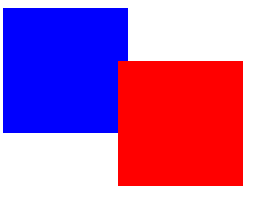
\includegraphics[scale=0.7]{img/C8/8-4/1.png}
\end{figure}

\begin{lstlisting}[style=htmlcssjs, title=olympic.html]
<!DOCTYPE html>
<html lang="en">
<head>
    <meta charset="UTF-8">
    <title>奥运五环</title>
    <link rel="stylesheet" type="text/css" href="olympic.css">
</head>
<body>
    <!-- 展示奥运五环的区域 -->
    <div class="stage">
        <div id="circle1"></div>
        <div id="circle2"></div>
        <div id="circle3"></div>
        <div id="circle4"></div>
        <div id="circle5"></div>
    </div>
</body>
</html>
\end{lstlisting}

\begin{lstlisting}[style=htmlcssjs, title=olympic.css]
* {
        margin: 0;
        padding: 0;
    }
    
    .stage {
        position: absolute;
        left: 50%;
        top: 50%;
        margin-left: -190px;
        margin-top: -93px;
        height: 185px;
        width: 380px;
    }
    
    #circle1,
    #circle2,
    #circle3,
    #circle4,
    #circle5 {
        position: absolute;
        width: 100px;
        height: 100px;
        border: 10px solid black;
        border-radius: 50%;
    }
    
    #circle1 {
        border-color: blue;
        left: 0;
        top: 0;
    }
    
    #circle2 {
        border-color: black;
        left: 130px;
        top: 0;
    }
    
    #circle3 {
        border-color: red;
        left: 260px;
        top: 0;
    }
    
    #circle4 {
        border-color: yellow;
        left: 65px;
        top: 70px;
    }
    
    #circle5 {
        border-color: green;
        left: 195px;
        top: 70px;
    }
\end{lstlisting}

\newpage